\documentclass{vgtc}                      % final (conference style)
%\documentclass[review]{vgtc}                 % review
%\documentclass[widereview]{vgtc}             % wide-spaced review
%\documentclass[preprint]{vgtc}               % preprint
%\documentclass[electronic]{vgtc}             % electronic version

\ifpdf
  \pdfoutput=1\relax
  \pdfcompresslevel=9 
  \pdfoptionpdfminorversion=7
  \ExecuteOptions{pdftex}
  \usepackage{graphicx}
  \DeclareGraphicsExtensions{.pdf,.png,.jpg,.jpeg} 
\else%
  \ExecuteOptions{dvips}
  \usepackage{graphicx}
  \DeclareGraphicsExtensions{.eps}
\fi

%% it is recomended to use ``\autoref{sec:bla}'' instead of ``Fig.~\ref{sec:bla}''
\graphicspath{{figures/}{pictures/}{images/}{./}}

\usepackage{microtype}
\PassOptionsToPackage{warn}{textcomp} 
\usepackage{textcomp}
\usepackage{amsmath}
\usepackage{mathptmx}
\usepackage{times}
\renewcommand*\ttdefault{txtt}
\usepackage{cite}
\usepackage{tabu} 
\usepackage{booktabs}

%% If you are submitting a paper to a conference for review with a double
%% blind reviewing process, please replace the value ``0'' below with your
%% OnlineID. Otherwise, you may safely leave it at ``0''.
\onlineid{0}

%% declare the category of your paper, only shown in review mode
\vgtccategory{Research}

%% allow for this line if you want the electronic option to work properly
\vgtcinsertpkg

%% In preprint mode you may define your own headline.
%\preprinttext{To appear in an IEEE VGTC sponsored conference.}





%% Paper title.
\title{SynMapN: Comparing Multiple Genomes}

\author{
Mingwei Li\thanks{e-mail: mwli@email.arizona.edu}
\and Carlos Scheidegger\thanks{e-mail: cscheid@cs.arizona.edu}
\and Eric Lyons\thanks{email: elyons.uoa@gmail.com}
\and Asher Keith Haug-Baltzell\thanks{email: ahaug@email.arizona.edu}
%TODO Eric and Asher, Heather, Sean?
}
\affiliation{\scriptsize University of Arizona}


%% A teaser figure can be included as follows, but is not recommended since
%% the space is now taken up by a full width abstract.
%\teaser{
%  \includegraphics[width=1.5in]{sample.eps}
% \caption{Lookit! Lookit!}
%}



%% Abstract section.
\abstract{
In this poster we give a study of visual exploration of data in the area of comparative genomics. We apply dimensionality reduction in visualizing comparison of many genomes (\autoref{fig:synmap_n}), to give genomicists a high-level overview of the genomes of his/her interest. We try to answer the question of how to provide visual guidance in studying the genetic relations of many genomes.
}


%% ACM Computing Classification System (CCS). 
%% See <http://www.acm.org/class/1998/> for details.
%% The ``\CCScat'' command takes four arguments.
%TODO how to generate this
\CCScatlist{ 
  %\CCScat{K.6.1}{Management of Computing and Information Systems}%
%{Project and People Management}{Life Cycle};
  %\CCScat{K.7.m}{The Computing Profession}{Miscellaneous}{Ethics}
}


%% Copyright space is enabled by default as required by guidelines.
%% It is disabled by the 'review' option or via the following command:
% \nocopyrightspace


%%%%%%%% START OF THE PAPER %%%%%%%%%%%%

\begin{document}
\firstsection{Introduction}
\maketitle
%% \section{Introduction} %for journal use above \firstsection{..} instead
In comparative genomics, one of the visual methods that helps studying the structural relations between two genomes is called syntenic dotplot \cite{syntenic_dotplot, synmap}.
It is a scatter-plot that depicts matched genes between two genomes, inferring regions, called synteny, that originated from the same ancestor. During the genetic analysis, a measure called synonymous mutation rate ($ks$) is computed. Synonymous mutation is a change if a DNA codon to one of its 'synonyms', which translates to the same amino acids thus does not change the protein this gene produce. $ks$ value is a rate of such mutation, normalized by gene sizes. Because those mutations are mostly unharmful and do not change environmental pressures or natural selections of the species, they can be seen as completely random events in a long period of time and thus can be used to predict evolutionary relations. The larger $ks$ value, the longer periods in time two genes are related.
%explain more on the plot, PARAPHRASE this:
%Each axis represents a sequence laid end-to-end, and each dot in the scatter-plot represents a putative homologous match between the two sequences
In the dotplot, two axes represent gene locations of two genomes respectively. Each dot on the plot represents a match between two genes. The color usually encodes $ks$ values.

In some ideal cases, a perfect alignment of two genomes can be observed by seeing a line along the diagonal of a plot, similar to a plot of function $y=x$. This means that the two entities in concern have same genes presented in order. More interesting events like duplication and inversion of genes can be easily spotted from the syntenic dotplot as well (\autoref{fig:dotplot_arabidopsis_marked}). In other cases, it is also common to see only sparse dots, indicating no significant alignment in the two genomes.

Although tools such as syntenic dotplots and MizBee \cite{meyer2009mizbee} and are widely useful, especially in comparing two genomes, there is not many tools in visualizing more than two genomes. In projects like 1000 genomes project \cite{1000genomes}, there is a demand of comparing and clustering many genomes. Adding one more axis of genome to make a 3D scatter plot, for example, may work in certain cases. We would see a line in  diagonal in comparison among human, chimpanzee and gorilla genomes\cite{synmap3durl}. However, it is not visually intuitive to find out complicated relations in 3 species in general. 
In fact, the user study of Tory et al. \cite{tory2007spatialization} showed that a 3D landscape works not as good as a 2D map in specific tasks such as search and point estimation. We concern about similar inefficiency and inaccuracy in visualizing relations among 3 species in a 3D scatterplot. Moreover, the idea of a 3D scatterplot does not generalize to more than 3 genomes.

%TODO citaion? what is paper first introduced scatterplot matrix?
Scatterplot matrix used in visualizing iris data can be adapted in comparing multiple genomes, with each subplot being a syntenic dotplot of two of the genomes. However, as the number of genomes increases, there is no way in telling the overall relation of genomes through a collection of synteny plots. The scatterplot matrix does not scale up well either.

We demonstrate some of our approaches of looking at genomic data. Specifically, we are interested in answering these questions through some visual guidance: What are the relationships of multiple genomes in the evolutionary process? Where in the underlying structure, such as chromosomes or gene ranges, caused their affinity? What parts of their DNA might share a same ancestor? Which of them are closer in time to the ancestor? Which of them share the same duplication or inversion events?

%We demonstrate an exploration of dimensionality reduction techniques to plot a map of multiple genomes, called SynMapN (\autoref{fig:synmap_n}), as an extension of SynMap \cite{syntenic_dotplot, synmap} which compares two genomes.


\begin{figure}[t]
 \centering
 \includegraphics[width=0.7\columnwidth]{scatterplot_matrix_human}
 \caption{A SynMapN plot of various species. Note the distant location of Escherichia coli (E.coli), the cluster of chimpanzee, gorilla and human, as well as the cluster of cat, dog and horse}
 \label{fig:scatterplot_matrix_human}
\end{figure}


\begin{figure}[t]
 \centering
 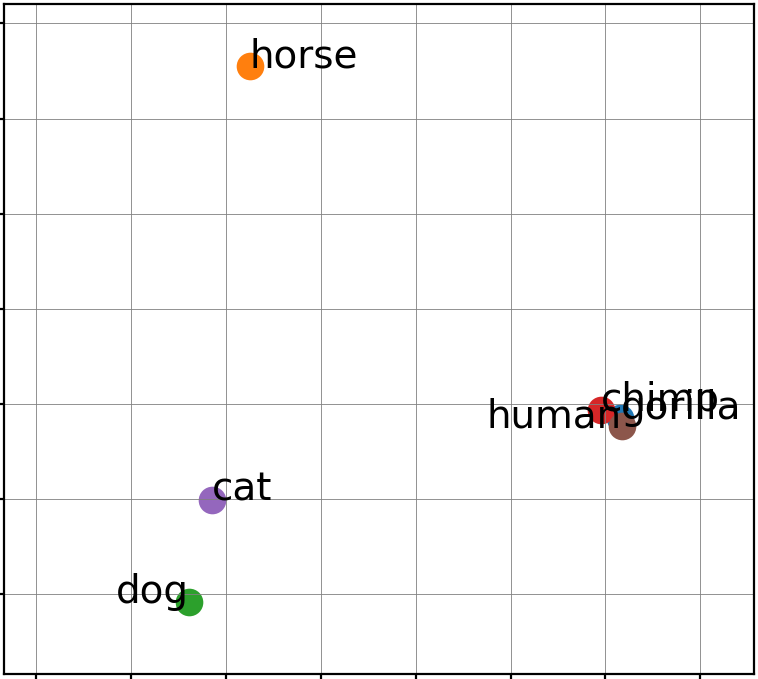
\includegraphics[width=0.7\columnwidth]{synmap_n}
 \caption{A SynMapN plot of various species. Note the distant location of Escherichia coli (E.coli), the cluster of chimpanzee, gorilla and human, as well as the cluster of cat, dog and horse}
 \label{fig:synmap_n}
\end{figure}


\begin{figure}[h]
 \centering
 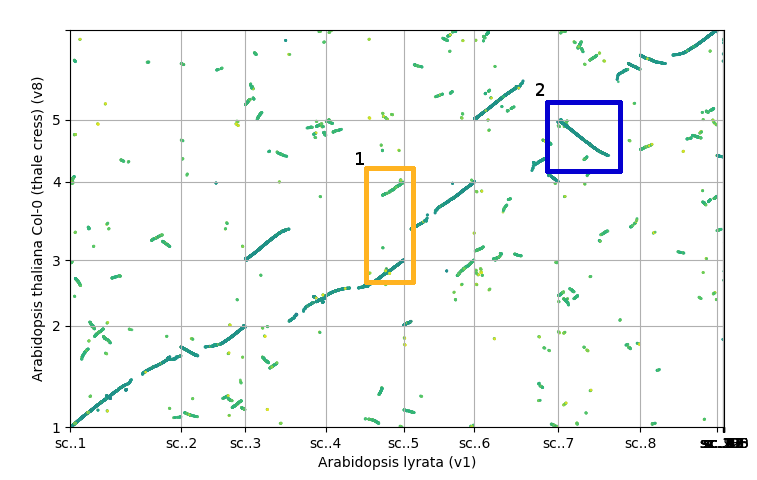
\includegraphics[width=0.8\columnwidth]{dotplot_arabidopsis_marked}
 \caption{A syntenic dotplot of Arabidopsis lyrata and Arabidopsis thaliana. The orange region 1 shows a duplication in Arabidopsis thaliana with respect to Arabidopsis lyrata. The blue region 2 shows an inversion. The image is regenerated by ks data downloaded from \cite{arabidopsisurl}.}
 \label{fig:dotplot_arabidopsis_marked}
\end{figure}


%\begin{figure}[h]
% \centering
% 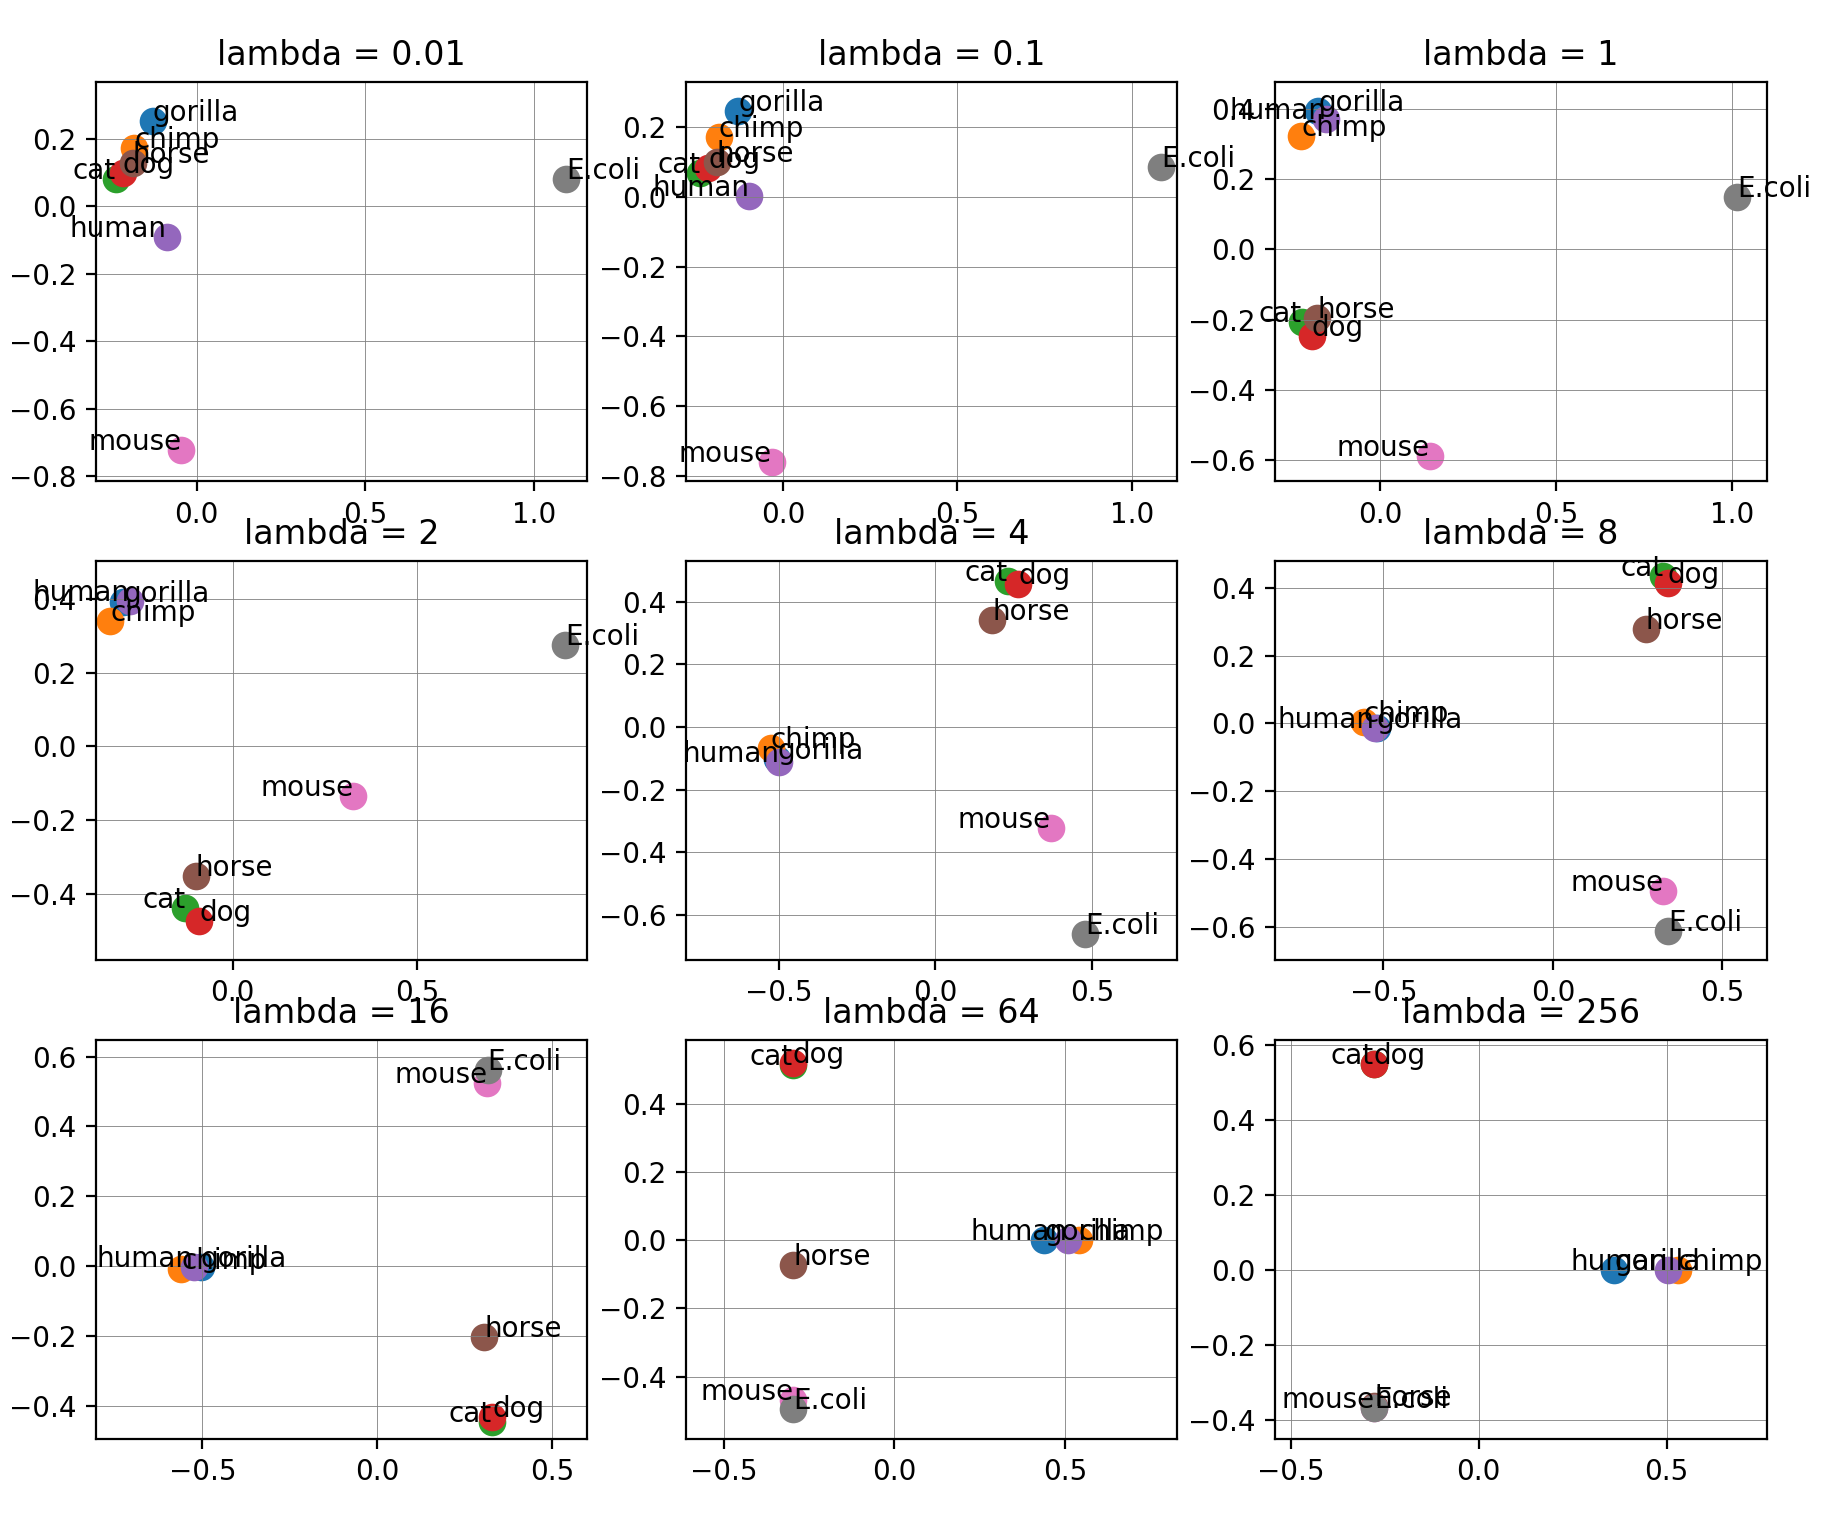
\includegraphics[width=\columnwidth]{lambda}
% \caption{lambda test}
% \label{fig:lambda}
%\end{figure}



 %TODO do this?
%\section{Related Works}
\section{Examples}
\autoref{fig:synmap_n} shows our first attempt of providing an overview of the genomes in concern. We define a similarity measure between two genomes, apply dimensionality reduction (Kernel PCA \cite{kernelpca}), and try to visualize the relationships among genomes of interest through a genomic map where distances between genomes encodes their affinity.

\begin{figure}[th]
 \centering
 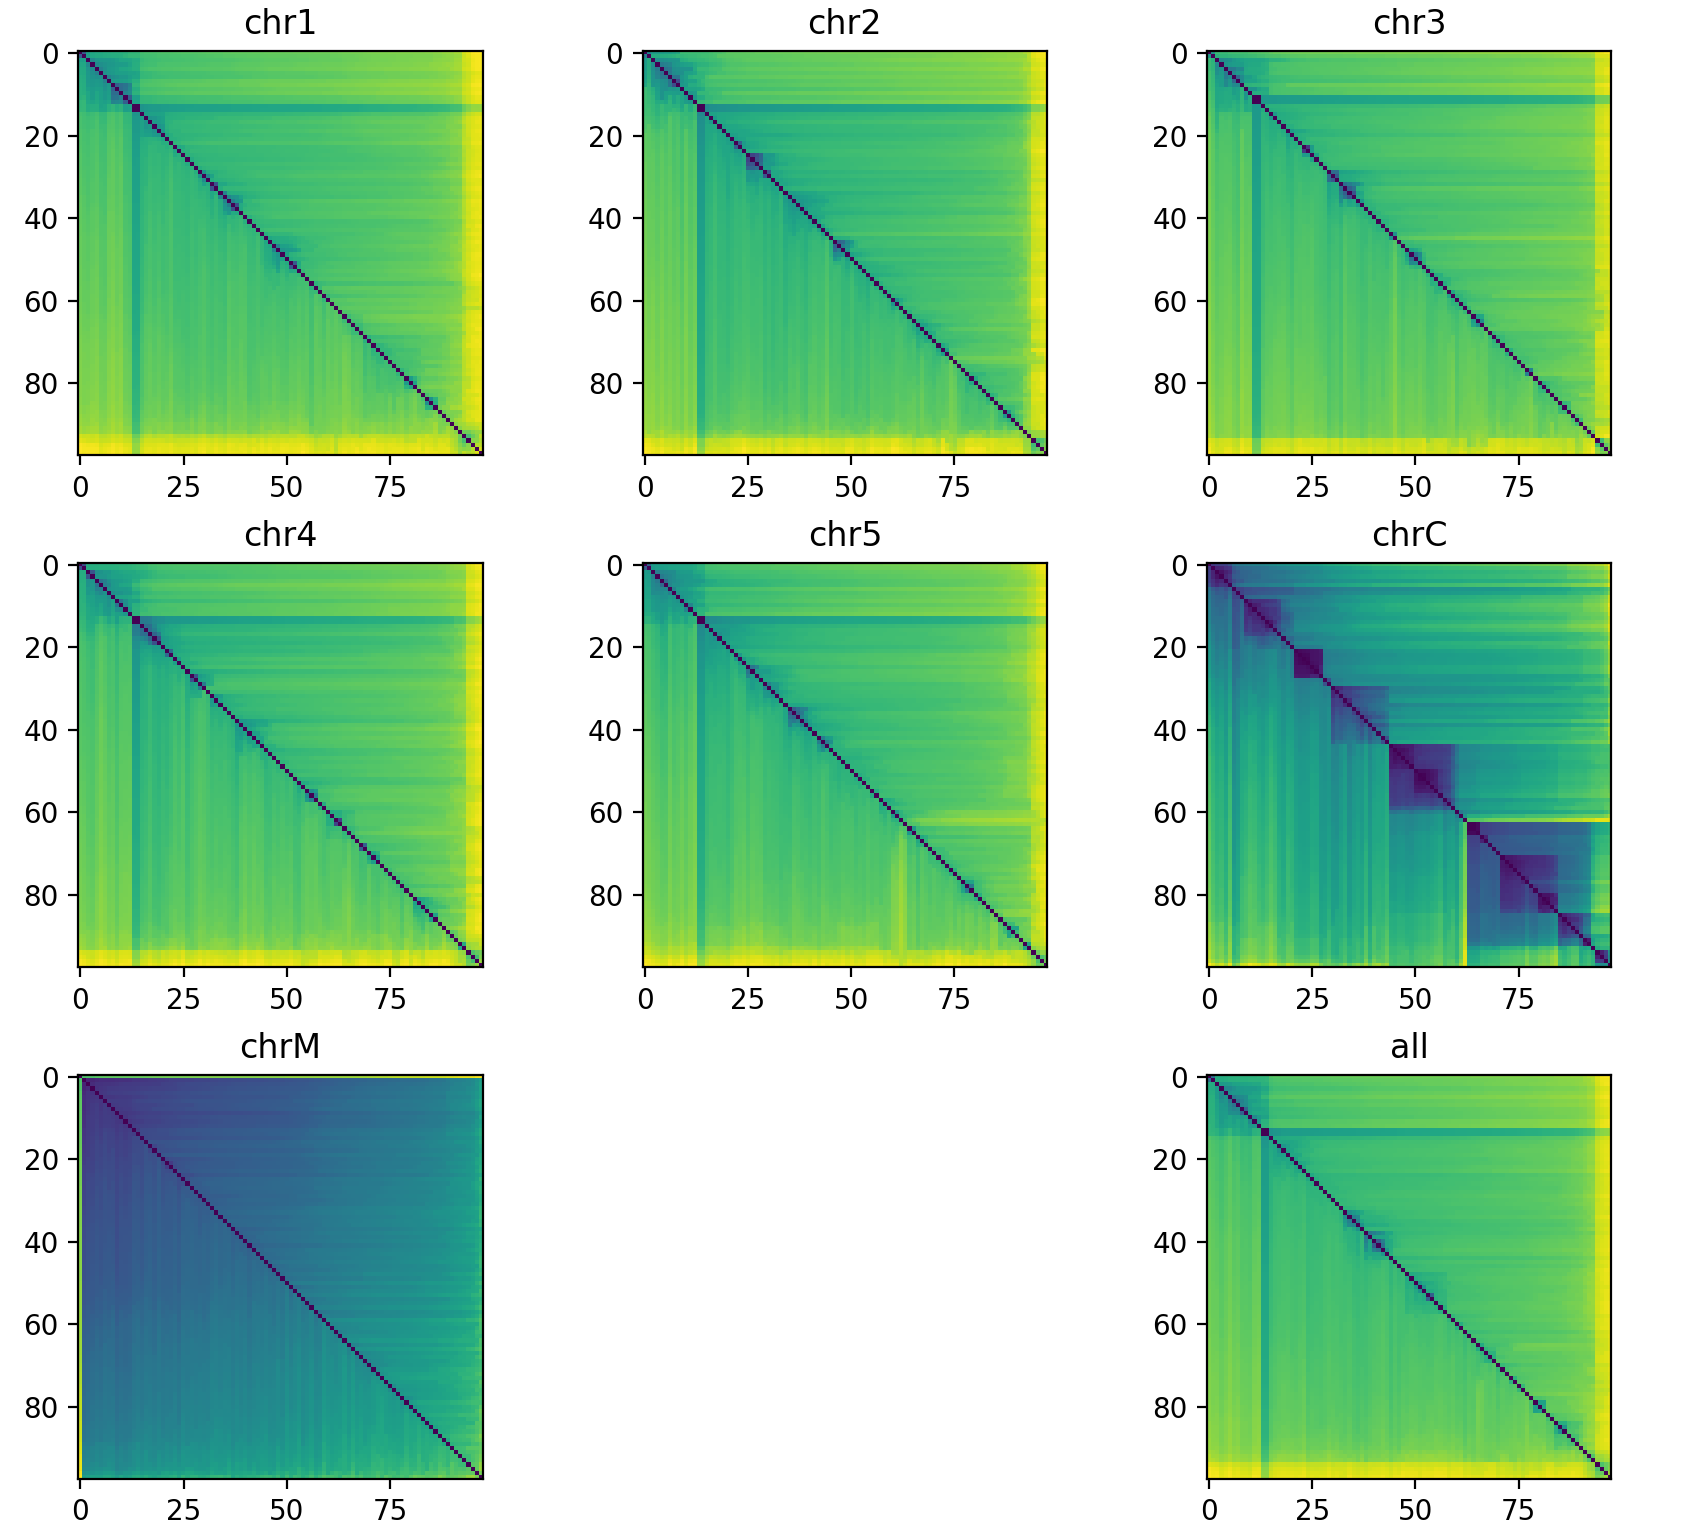
\includegraphics[width=0.8\columnwidth]{chromosomes_matrix}
 \caption{Distance matrices of 97 Arabidopsis thaliana of different ecotypes. Eight subplots are 7 individual chromosomes and a sum of them. Clusters and outliers can be spotted in chromosome C (subplot \#6)}
 \label{fig:chromosomes_matrix}
\end{figure}

\begin{figure}[th]
 \centering
 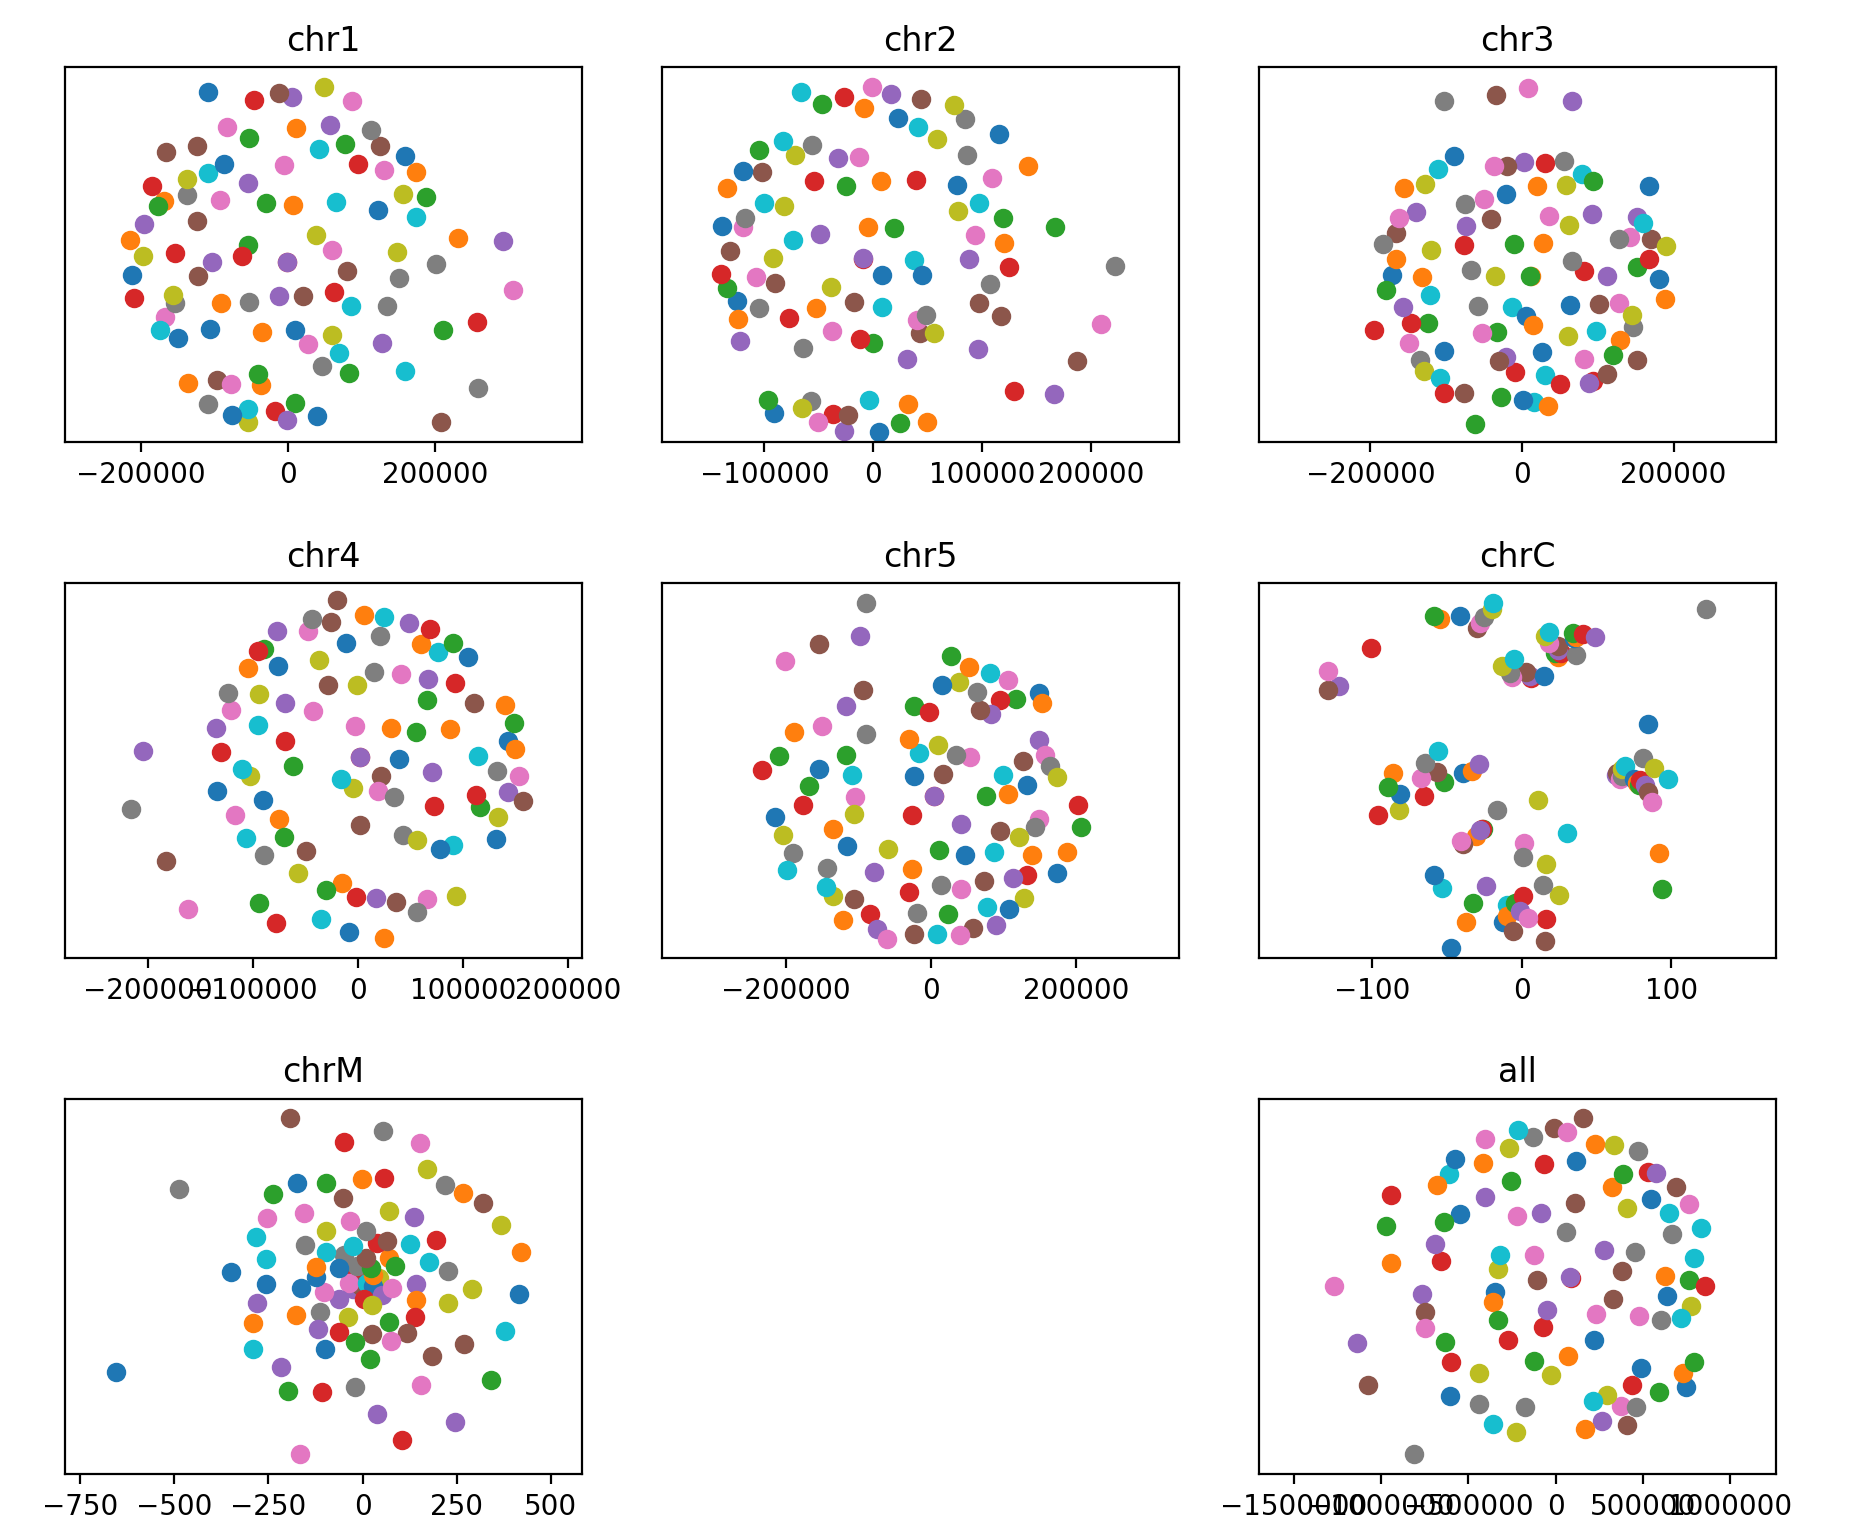
\includegraphics[width=0.8\columnwidth]{chromosomes_scatter}
 \caption{MDS plots of 97 Arabidopsis thaliana of different ecotypes.}
 \label{fig:chromosomes_scatter}
\end{figure}

\autoref{fig:chromosomes_matrix} and \autoref{fig:chromosomes_scatter} show distance matrices and scatterplots (coordinates computed from MDS) of species from another dataset. The genomes are Arabidopsis of different ecotypes. When we break the entire genome into individual chromosomes and try to compute their pairwise edit distances, we see clusters in small chloroplast chromosomes (chrC, subplot \#6 in \autoref{fig:chromosomes_matrix} and \autoref{fig:chromosomes_scatter}). We can also see some common outliers among other plots.

%TODO to be trimed
\section{Method}
In the process of drawing a SynMap of two genomes, the program computes a measure called synonymous mutation rate ($ks$) describing a matching score for each pair of aligned genes between two genomes. This score ranges from $0$ to $+\infty$, or arbitrary large number in data, with $0$ means perfect alignment and infinity indicates no alignment or an error. We want to utilize these measures to build a notion of distance between two genomes. 

For example, when comparing two genomes of human and chimp, we are given IDs of gene pairs and their synonymous mutation rate, denoted by $ks$, which can be seen as a measure of distance (\autoref{tab:table_input_example})

\begin{table}[h!]
\centering
\caption{Data Input File}
\label{tab:table_input_example}
\begin{tabular}{cc|c}
\toprule
%\multicolumn{2}{c}{Gene labels} &\\
%\midrule
Human & Chimpanzee & $ks_i$\\
gene ID & gene ID & \\
\midrule
h1 & c1 & 0.0056\\
h2 & c2 & 72.6574\\
... & ... & ...	\\
\bottomrule
\end{tabular}
\end{table}

Now we want to find a function of many ks values that describes the distance between two genomes or equivalently, a notion of similarity or kernel between two entities.
\begin{align}
similarity(Human, Chimp) = g(ks_1,ks_2...)
\end{align}


Generally the gene IDs in such table may be duplicated, indicating a match of a single gene from one genome with multiple genes in the other genome (duplication). To formalize the computation, we put $ks$ values in matrix form

%ks_{2,1} & ks_{2,2} & ks_{2,3} & \dots & ks_{2, c}\\
%matrix representation
$$K = 
\begin{bmatrix}
ks_{1,1} & ks_{1,2} & \dots & ks_{1, c}\\
\vdots & \vdots & \ddots & \vdots \\
ks_{h,1} & ks_{h,2} & \dots & ks_{h, c}\\
\end{bmatrix}
$$

Where $ks_{1,1}$ stores the ks value between the first gene of human and the first gene of chimpanzee, and so on. The indices of rows and columns are in the order of gene locations in ordered chromosomes.
%, chromosomes are ordered in a natural order to genomicists. 
$h$ and $c$ are gene counts of human and chimpanzee respectively. One can think of $K$ as an image data of the SymMap plot (\autoref{fig:dotplot_arabidopsis_marked}).

Now we want a function of $K$ that outputs a scalar value to describe the similarity between two genomes.
\begin{align}
similarity(Human, Chimp) = f(K)
\end{align}

%TODO include this?
%Intuitively we want a measure similar to the dot product of vectors of unit length, which encodes cosine of the angle between the two vectors. Moreover, the dot products should better not generating any negative values since there is not a notion of 'negative of a human' among species.

To define a function so that comparison of a genome to itself gives a similarity measure close to $1$, we used $f$ to compute kernels between any two genomes, which are later used to plot \autoref{fig:synmap_n}
\begin{align}
f(K) = \frac{\sum_{i,j} e^{-\lambda K_{ij}}}{\sqrt{c \times h}}
\end{align}
Where $\lambda$ is a scalar constant related to sensitivity of the similarity measure. $c$ and $h$ are the gene counts defined before. 

Once we have the pairwise distances among multiple genomes (stored in matrix $M$), we have an implied space and then we project it onto a 2D screen using Kernel PCA.
Let $M$ be the matrix of similarities of multiple genomes where each entry is computed by function $f$ defined above. Note that this is a symmetric matrix with diagonal entries set to $1$, indicating complete identity in similarity measure of each genomes with respect to itself.
$$M = 
\begin{bmatrix}
f_{human, human} & f_{human, chimp} & f_{human,cat} & \dots \\
f_{chimp, human} & f_{chimp, chimp} & f_{chimp, cat} & \dots \\
\vdots & \vdots & \vdots & \ddots \\
\end{bmatrix}
$$
We then treat it as a kernel matrix and feed it into existing Kernel PCA algorithms and plot the first two principle components, which is shown in \autoref{fig:synmap_n}
\section{Other Examples}

\begin{figure}[h]
 \centering
 %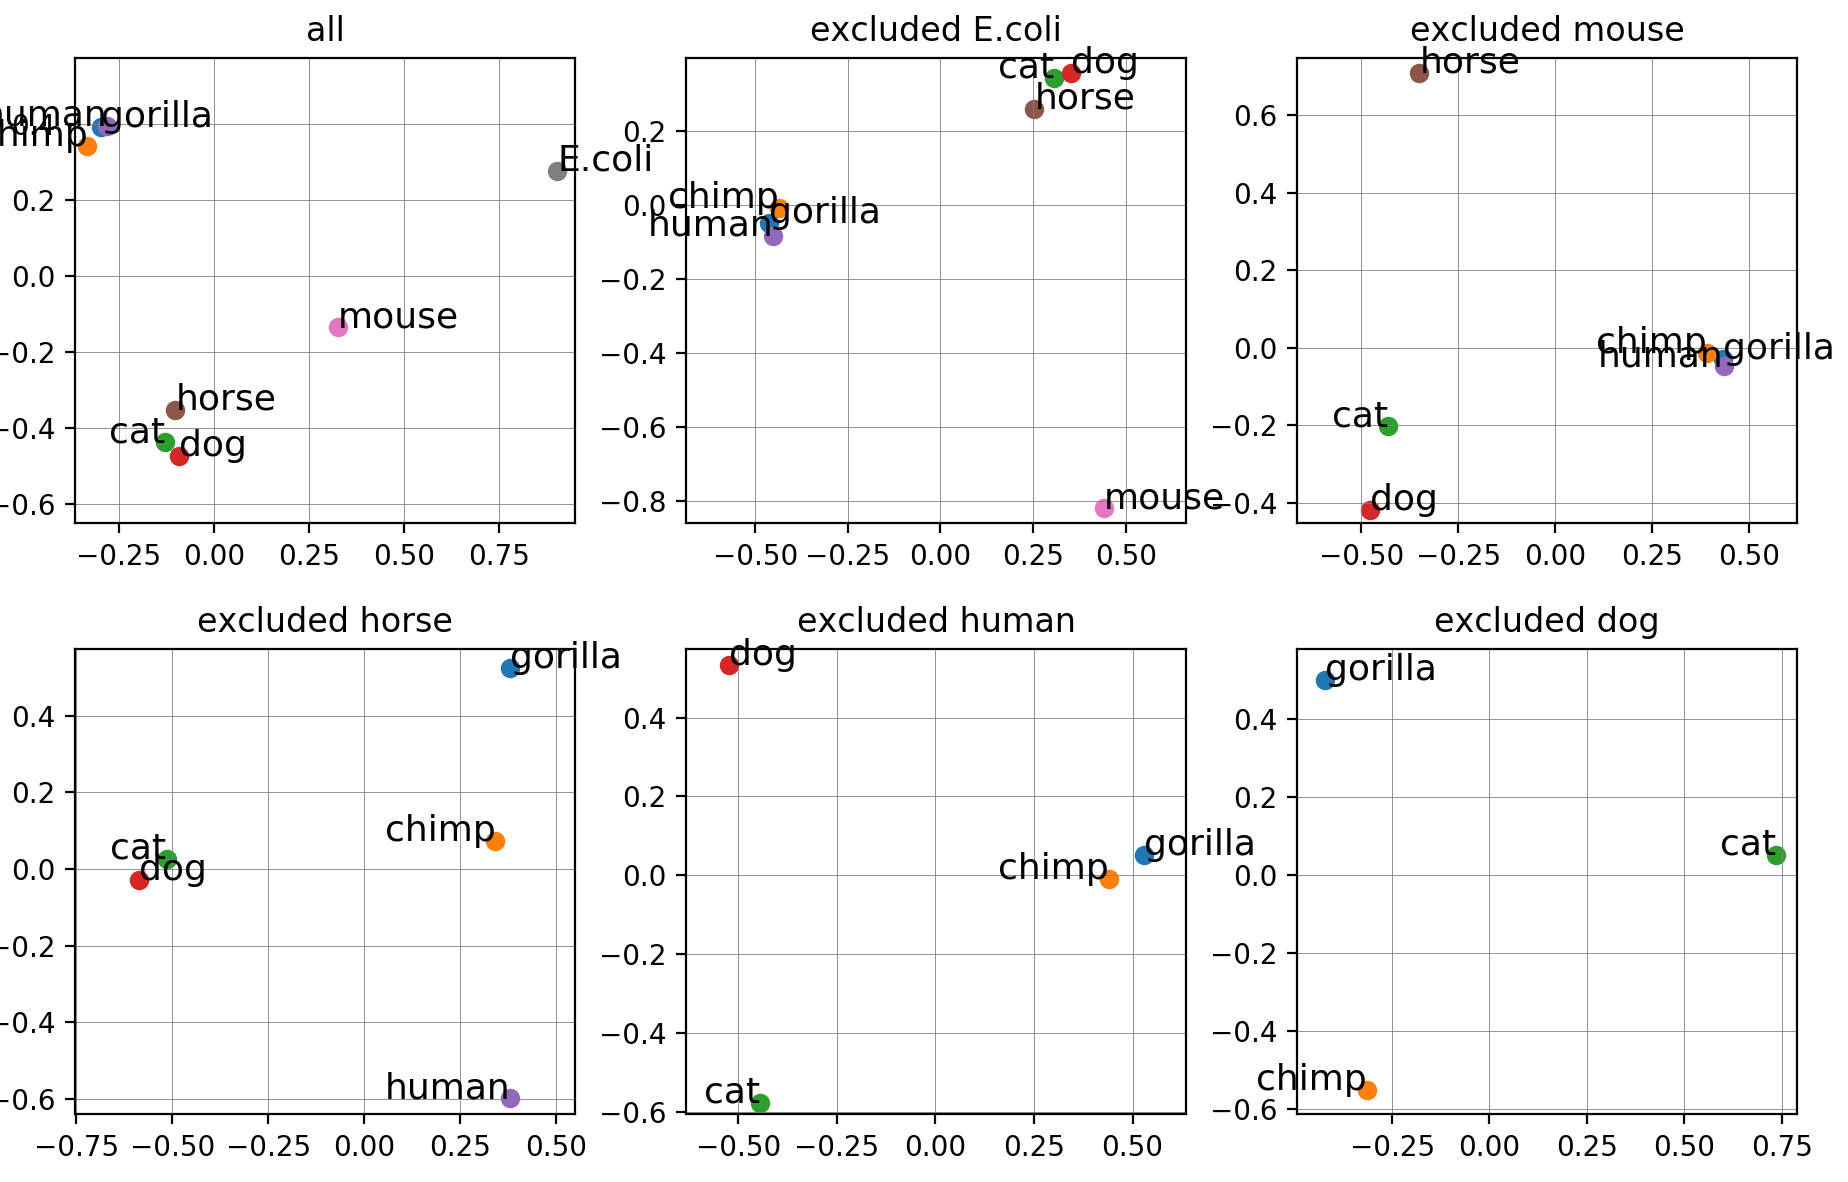
\includegraphics[width=0.8\textwidth]{subset}
 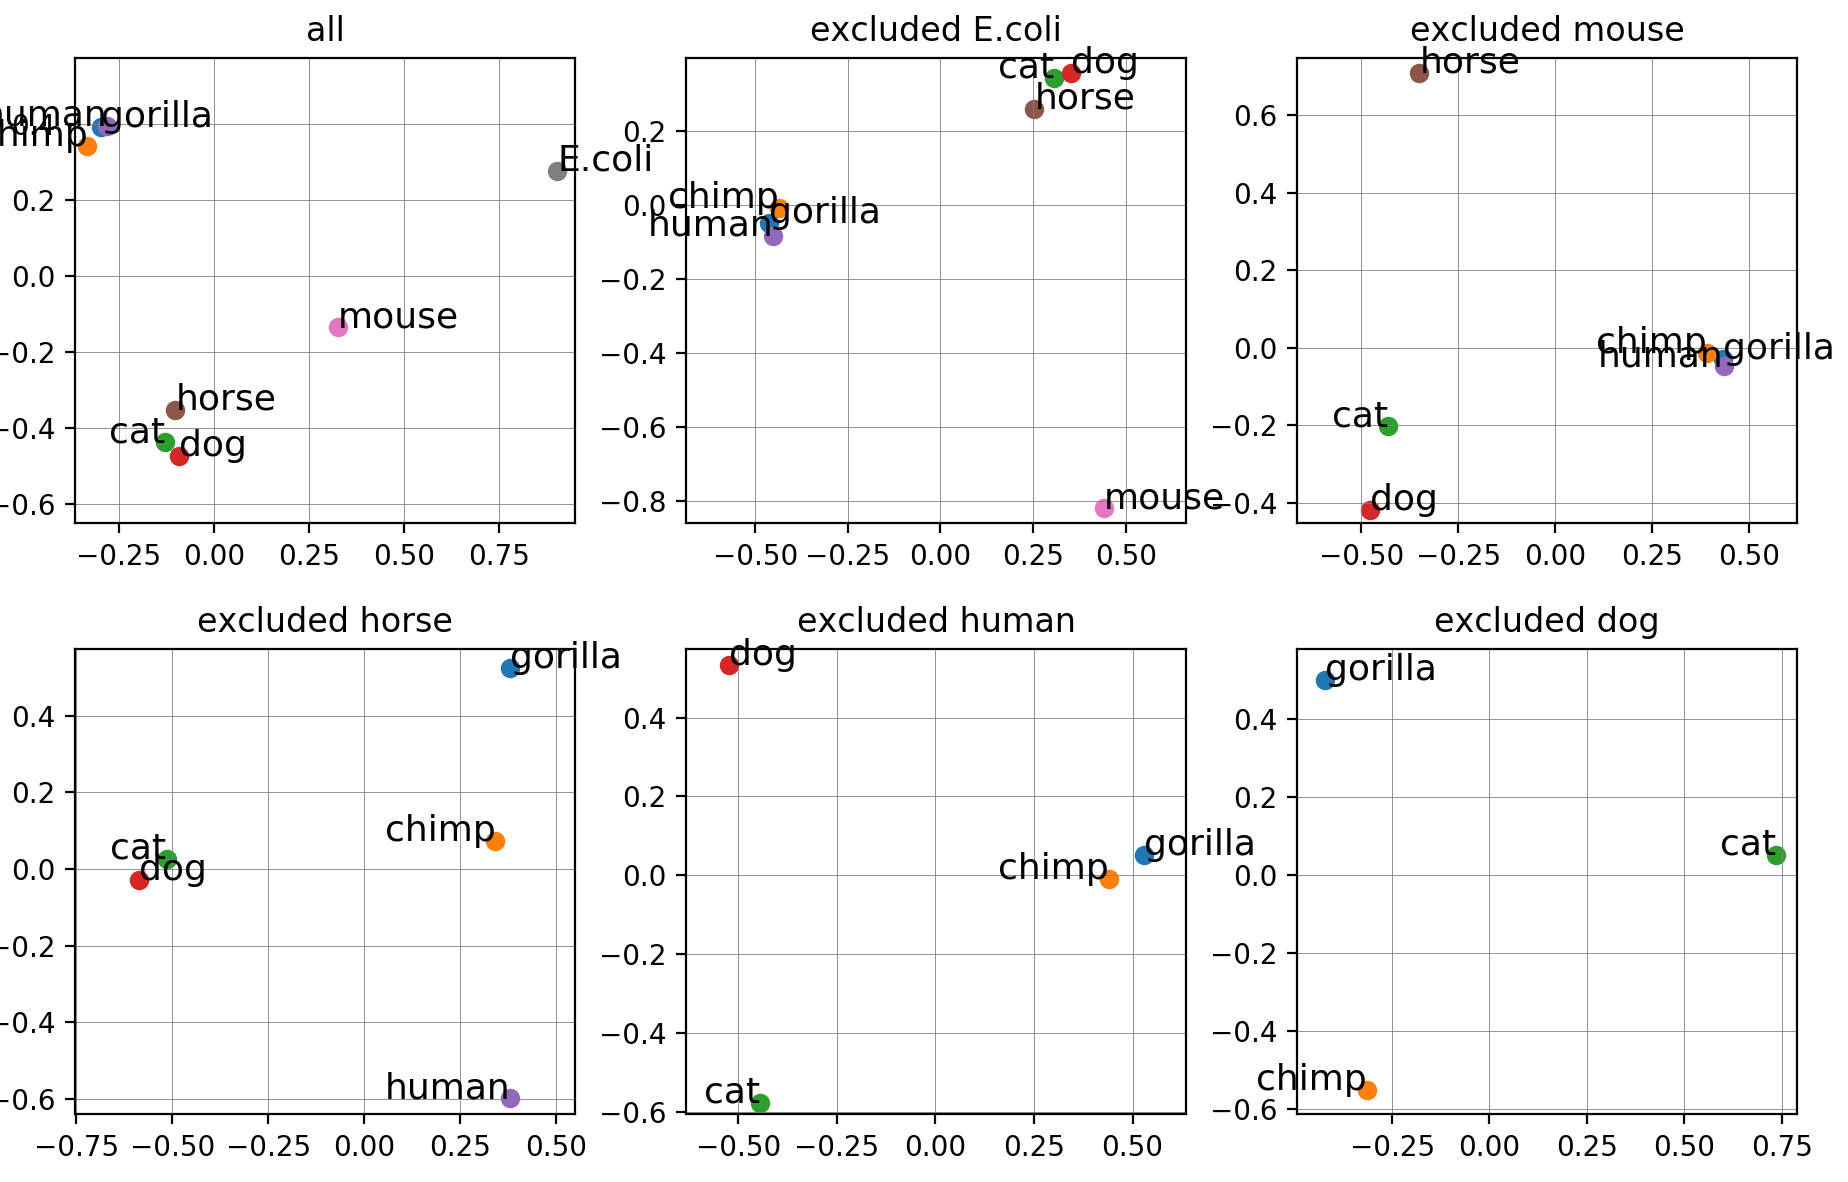
\includegraphics[width=\columnwidth]{subset}
 \caption{A SynMapN plot with subsets of species concerned. The similarity measure of certain pairs are the same among all plots above so the distance encoded are consistent.}
 \label{fig:subset}
\end{figure}

In addition to the example plot in \autoref{fig:synmap_n}, we explore different subsets of the genomes among the genomes we concerned to show the capacities and constraints of SynMapN. 
%We show another distance measure used for a different dataset of more similar species represented in single-nucleotide polymorphism (SNP) data format.

%different lambda values and diferent subset of genomes
%closely related genomes, different approach

Plots in \autoref{fig:subset} shows subsets of the genomes we concerned with one genome excluded a time. The similarity of each pair of genomes are consistent among all the plots so the distances in the implied high dimensional space remains the same. But note that a 2D Kernel PCA plot reveals more of the true distances wist respect to an outlier through a certain plot, while potentially shrink the pairwise distances among other points. When an outlier is removed from the input of Kernel PCA in the next plot, another outlier shows up, indicating that previous plot did not show the true distance of the later outlier. For example, plot 2 shows affinity of horse, cat and dog, while with mouse excluded in plot 3, horse moves away from the cat-dog cluster. 

SynMapN gives an overview of genomes while ignoring the details of the comparison. The detailed patterns within two genomes comparison such as inversions and duplications are not shown in SynMapN. The other restriction lies on the limitation of dimensionality reduction method we use. Kernel PCA and Classical MDS\cite{mds} are essentially linear projections that preserves the pairwise distances globally, so the distant dots reflects the dissimilarities of the entities while the closed dots may only be an artifact of the projection, thus misleadingly reflects closeness of entities in similarity. So SynMapN at this stage is very useful in finding one specie that are most dissimilar from the others while the clustering it plots does not always reflect the truth.



%(more on SNPs dataset?)

  
\section{Future Works}
In a complete visualization system, we expect to enable users to navigate through various visualizations for different levels of details, from high level SynMapN to very detailed comparison of two specific genomes in SynMap. To further increase the number of levels, we can split genomes into individual chromosomes and compare them in SymMapN. We are also exploring the possibilities of capturing certain features in a SynMap plot, for example, the diagonal alignments or anti-diagonal alignments, using image processing. More improvements on interaction can be done through studying observation level interactions \cite{endert2011observation}, to enable users to specify desired clustering criteria through dragging points in the plot. 

%TODO do this?
%\section{Conlcusion}



%% if specified like this the section will be committed in review mode
\acknowledgments{
%The authors wish to thank A, B, C. This work was supported in part by
%a grant from XYZ.
}

%\bibliographystyle{abbrv}
\bibliographystyle{abbrv-doi}
%\bibliographystyle{abbrv-doi-narrow}
%\bibliographystyle{abbrv-doi-hyperref}
%\bibliographystyle{abbrv-doi-hyperref-narrow}

\bibliography{mybib}
\end{document}
